\chapter{Implementierung} \label{chp:implementation}

\section{Design Prototyp}
Um der Konfigurationsoberfläche ein Aussehen verleihen zu können, wird zunächst ein Design-Prototyp erstellt. Hierzu werden alle Komponenten aufgelistet, welche in diesem Projekt Verwendung finden.

\begin{itemize}
    \item Titelleiste mit Menüunterpunkt zum Hinzufügen neuer Endpunkte
    \item Aufklappbare Endpunktliste. Beim Aufklappen sollen Informationen zum Endpunkte ersichtlich sein.
    \item Neuer-Endpunkt/Endpunkt bearbeiten Dialog
\end{itemize}

Der erste Prototyp wird mit Adobe Illustrator\footnote{https://www.adobe.com/de/products/illustrator.html} erstellt. Das Design, wird absichtlich schlicht und übersichtlich gehalten.

Im oberen Teil lässt sich die Titelleiste erkennen, welche auch als Menü fungiert. So lässt sich mit dem Klick auf den rechten Menüpunkt zum Beispiel ein Fenster öffnen. Hier kann dann ein neuer Endpunkt manuell erstellt oder mittels \gls{csv}-Datei angelegt werden. Nach erfolgreichem Anlegen eines neuen Endpunkts erscheint dieser wiederrum in der Liste im Hauptmenü. Diese Einträge lassen sich ausklappen, sodass sichtbar wird, wie diese Endpunkte zu verwenden sind. Entsprechende \gls{http}-Methoden werden hier ersichtlich sein. Zusätzlich wären in diesem Teil auch noch weitere Bedienelemente denkbar, welche das Löschen oder Anzeigen der Endpunkte ermöglicht.

Die Anzeige der Endpunkte kann zum Beispiel in Tabellenform erfolgen. Die konkrete Implementierung wird im Kapitel \ref{sec:frontend} illustriert.

\begin{figure}[h]
    \centering
    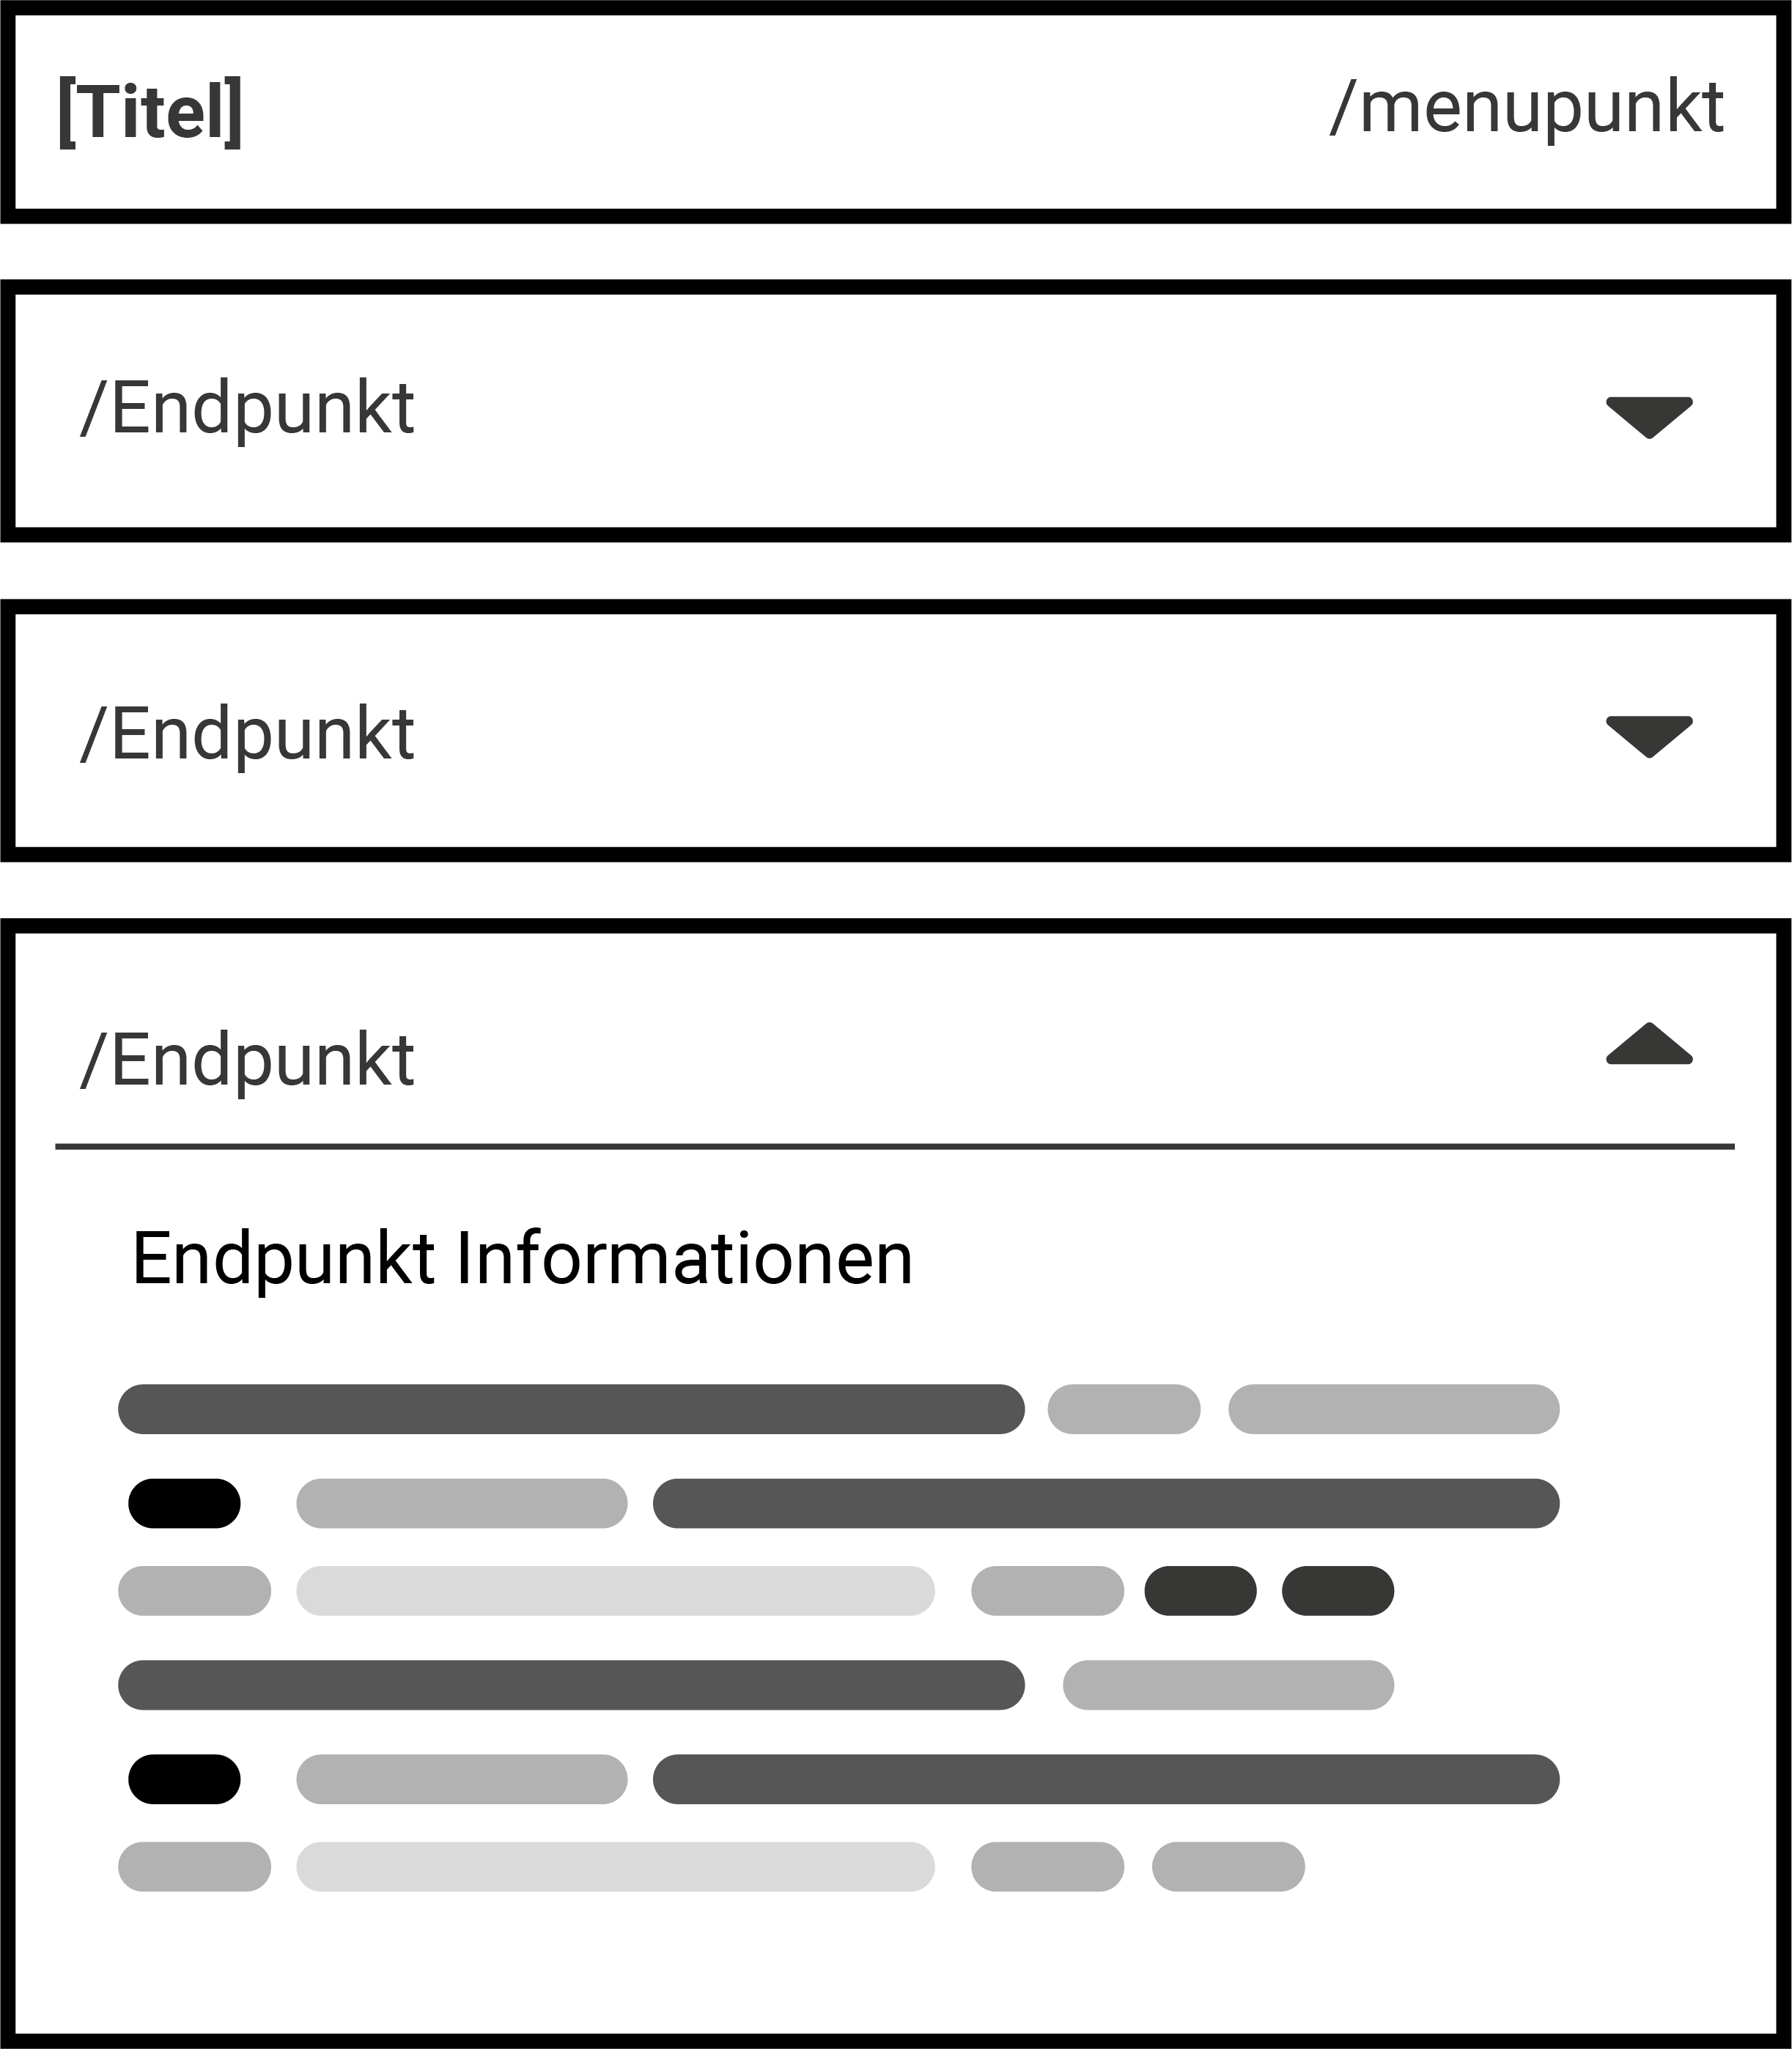
\includegraphics[width=0.6\textwidth]{figures/mock-up.png}
    \caption{Design-Prototyp}
    \label{fig:mock-up}
\end{figure}

\section{Backend} \label{sec:backend}

\subsection{Express.js}
Das sehr bekannte Framework \textit{express.js} wird verwendet, um Endpunkte der \gls{restapi} bereitzustellen. Auch das im nächsten Kapitel zu entwickelnde Frontend kann mittels dieses Frameworks bereitgestellt werden. Es bietet einige rubuste Module für die Entwicklung von Webapplikationen. In dem Buch \textit{REST API Development with Node.js} wird ein Generator verwendet, welcher das initiale Aufsetzen des Projektes und der Ordnerstrukturen stark vereinfacht. Der sogenannte \textit{express-generator} füllt ein leeres Projekt mit Ordnern, Dateien und beispielhaftem Code \cite{Doglio.2018}. Auf diesen Generator wird jedoch verzichtet, um die Entwicklung des Projektes genauer Untersuchen zu können und selbst die geeignete Ordnerstruktur anzulegen. 

Die Struktur wurde bereits im Kapitel \ref{subsub:system-architectuere} festgelegt. Auf dieser aufbauend werden die einzelnen Komponenten im Folgendem näher betrachtet.


\subsection{Controller}
Controller werden in diesem Projekt verwendet, um eingehende \gls{http}-Anfragen zu validieren und die \gls{http}-Schicht von der Business-Logik zu trennen. Wenn eingehende Anfragen nicht im richtigen Format vorliegen werden sie an dieser Stelle direkt mit einem entsprechenden Status-Code und eine Mitteilung beantwortet. 

\begin{figure}[h]
    \centering
    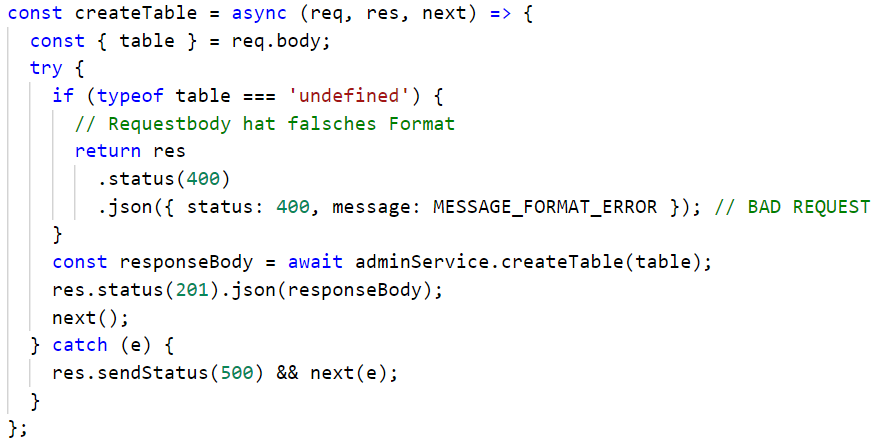
\includegraphics[width=0.8\textwidth]{figures/code-controller.png}
    \caption{createTable Methode des Admin-Controllers}
    \label{fig:createTable-controller}
\end{figure}

In der Abbildung \ref{fig:createTable-controller} lässt sich eine solche Prüfung erkennen. Zunächst wird mit
\begin{verbatim}
    const { table } = req.body;
\end{verbatim}
aus dem, in der Anfrage übergebenem, \gls{json}-Body das Objekt \textit{table} ausgelesen. im nächsten Schritt wird dann geprüft, ob dieses Objekt definiert ist. Im Negativfall wird direkt eine Antwort mit dem Status-Code 400 generiert. Dieser steht für \textit{BAD REQUEST}; also fehlerhafte Anfrage. Ist das Objekt \textit{table} jedoch definiert, wird es zur weiteren Verarbeitung an die Business-Logik weitergereicht. 
\subsection{Services}
Im Ordner \textit{Services} befindet sich die Business-Logik. Eingehende Anfragen werden aufbereitet, an die Datenbank gesendet und im \gls{json}-Format wieder an die \textit{Controller}-Schicht zurückgegeben. 

\begin{figure}[h]
    \centering
    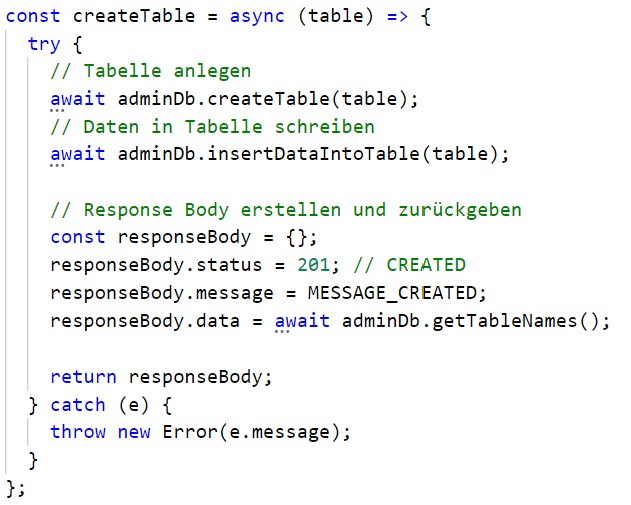
\includegraphics[width=0.6\textwidth]{figures/code-services.png}
    \caption{createTable Methode des Admin-Services}
    \label{fig:createTable-services}
\end{figure}

In Abbildung \ref{fig:createTable-services} wird das vorherige Beispiel zum Erstellen einer Tabelle wieder aufgegriffen. Die Funktion nimmt eine Tabelle im folgenden Format entgegen:

\begin{verbatim}
    {
        table: {
            name: "Tabellenname (Pfadname)",
            header: ["Erster Spaltenname", "Zweiter Spaltenname"....],
            data: [
                ["Erste Reihe 1", "Erste Reihe 2"....],
                ["Zweite Reihe 1", "Zweite Reihe 2"....]
            ]
        }
    }
\end{verbatim}

Diese Struktur wird nicht weiter verändert und über die Modul-Methode \textit{adminDb.createTable(table)} respektive \textit{adminDb.insertDataIntoTable(table)} an die nächste Schicht weitergegeben. Nach erfolgreicher Ausführung wird eine Antwort generiert. Hierzu wird ein neues Objekt erstellt: \textit{responseBody}. Diesem Objekt werden Attribute hinzugefügt.

\begin{itemize}
    \item responseBody.status: Der zurückzugebene Status-Code (in diesem Fall 201 CREATED)
    \item responseBody.message: Eine textuelle Nachricht um anzuzeigen, dass die Ressource erfolgreich erstellt wurde.
    \item responseBody.data: Hier werden noch einmal von der Model-Ebene alle Tabellennamen abgerufen, um sie mit der \gls{json}-Formatierten Antwort an die Controller-Ebene zurückzugeben. 
\end{itemize}

\subsection{Model}
Im Modul \textit{DB} (in diesem Ffalle das Datenmodell) findet die Kommunikation mit der zugrundeliegende \textit{sqlite}-Datenbank statt. Anfragen aus der Services-Schicht werden entgegengenommen, verarbeitet und beantwortet. Um das Beispiel \textit{createTable} weiterhin zu verfolgen, werden aus diesem Modul drei verschiedene Methoden vorgestellt. 

\begin{figure}[h]
    \centering
    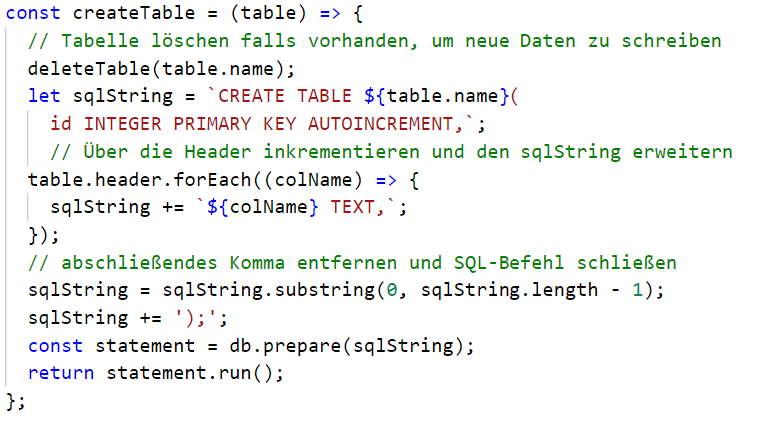
\includegraphics[width=0.8\textwidth]{figures/code-model-createTable.png}
    \caption{createTable Methode des Admin-Models}
    \label{fig:createTable-model-createTable}
\end{figure}

Die \textit{createTable}-Methode in Abbildung \ref{fig:createTable-model-createTable} nimmt ein Objekt im schon bekannten Format entgegen. Eine eventuell bestehende Tabelle wird zunächst entfernt. Dadurch kann diese Funktion auch genutzt werden, um änderungen in die Datenbank zu schreiben. 

\begin{figure}[h]
    \centering
    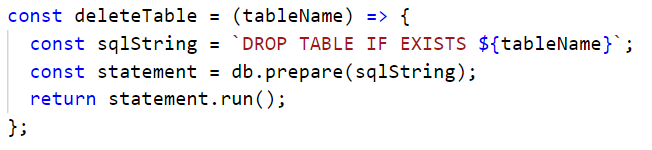
\includegraphics[width=0.8\textwidth]{figures/code-model-deleteTable.png}
    \caption{deleteTable Methode des Admin-Models}
    \label{fig:createTable-model-deleteTable}
\end{figure}

Diese Funktion ist in Abbildung \ref{fig:createTable-model-deleteTable} zu sehen und ist eine Ummantelung des \gls{sql}-Statements \textit{DROP TABLE IF EXISTS tabellenname} \cite{Gerner.2006}.


\begin{figure}[h]
    \centering
    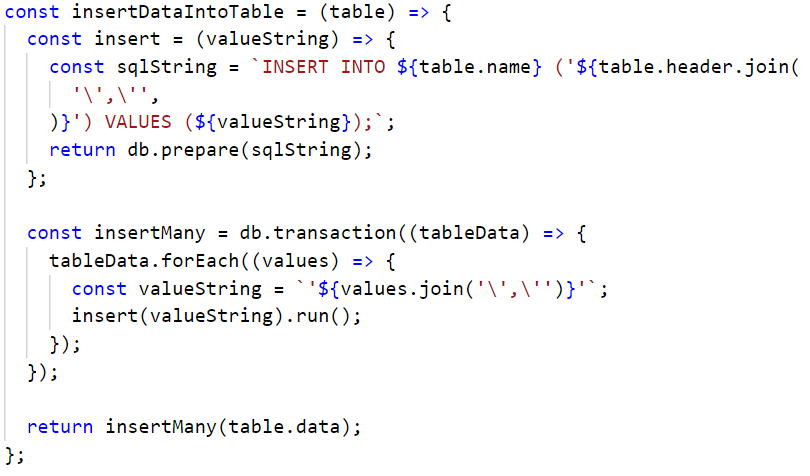
\includegraphics[width=0.8\textwidth]{figures/code-model-insertDataIntoTable.png}
    \caption{insertDataIntoTable Methode des Admin-Models}
    \label{fig:createTable-model-insertDataIntoTable}
\end{figure}

Etwas komplexer dagegen ist die Funktion \textit{insertDataIntoTable} (Abbildung \ref{fig:createTable-model-insertDataIntoTable}), welche ebenfalls das Objekt \textit{table} entgegennimmt. Diese Funktion besteht aus zwei Unterfunktionen.
Die Unterfunktionen \textit{insert} wird für jede anzulegende Tabellen-Zeile von insertMany aufgerufen. Hier wird ein \gls{sql}-Statement geformt \cite{Gerner.2006}:
\begin{verbatim}
    INSERT INTO tabellenname ('Spaltenname 1', 'Spaltenname 2'....) 
    VALUES ('Wert 1 Zeile n', 'Wert 2 Zeile n'....);
\end{verbatim}

Nach der Formung wird die gebildete Zeichenkette mit der \textit{.run()} Funktion auf der Datenbank ausgeführt. Dieser Vorgang wird so oft wiederholt, wie Zeilen mit übergeben wurden.

\subsection{Routes, Konstanten und app.js}
In diesem Unterkapitel werden die kleineren Module behandelt. Das Modul \textit{Routes} beinhaltet alle Endpunkte des Systems; sowohl die der Konfigurationsoberfläche als auch die generischen Endpunkte des Clients. Wie in Abbildung \ref{fig:routes} zu Erkennen, wird bei den Client-Routen der Platzhalter * genutzt. Somit wird hier jeder Aufruf der \gls{url}
\begin{verbatim}
    https://localhost:3000/api/
\end{verbatim}
abgefangen und verarbeitet. Auch Suchanfragen, sogenannte \textit{search querys}, werden hier berücksichtigt. Das Auslesen und Formatieren der Anfragen geschieht auf den unteren Ebenen (Controller, Services). 
\begin{figure}[h]
    \centering
    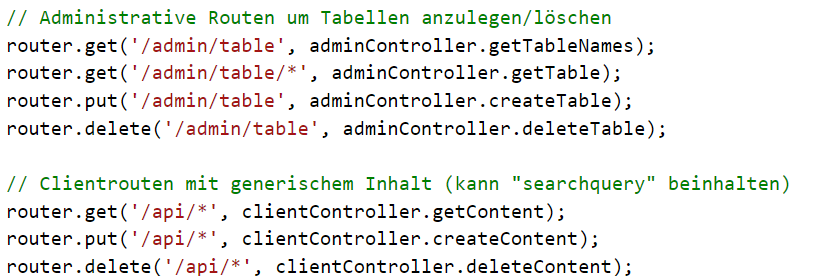
\includegraphics[width=0.8\textwidth]{figures/code-routes.png}
    \caption{Alle Routen des Systems}
    \label{fig:routes}
\end{figure}

Standard-Nachrichten, Ports und der App-Name werden im Modul \textit{Constants} aufbewahrt, somit sind diese global an jeder Stelle des Projekts verfügbar.
\\
Eine weitere wichtige Schlüsseldatei bildet die \textit{app.js}. In dieser Datei wird der \textit{express.js}-Server gestartet und mit den eben angeführtem Routen verbunden. Auch die statische Bereitstellung des Frontends  wird hier ausgeführt. Dies wird im Folgenden Kapitel näher beschrieben.

\section{Frontend} \label{sec:frontend}

\subsection{Bereitstellung und Modularisierung}

Das Frontend (die Benutzeroberfläche) mit der die lokale  \gls{restapi} angepasst wird ist eine reguläre Webseite, welche auf das Backend über die administrativen \gls{api} Schnittstellen zugreift. Die Ordner-Struktur ist relativ simpel gehalten. So gibt es einen Wurzelordner in dem sich die Hauptseite befindet (index.html) und drei Unterordner - \textit{css}, \textit{js} und \textit{assets}. 

Der Ordner \textit{js} beinhaltet JavaScript Dateien, welche die Modularisierung und die Kommunikation mit dem Backend übernehmen. In dessen Unterordner modules befinden sich Module, welche zur Laufzeit geladen werden. Dieses Prinzip ist ein relativ neues JavaScript-Feature und wird von allen modernen Browsern nativ unterstützt.

Durch die Modularisierung müssen nicht mehr alle Code-Teile eines Projekts in einer Datei gespeichert werden, 
sondern werden dynamisch importiert wenn nötig. \cite{Mozilla.2020}

Die Module sind wie folgt unterteilt:

\begin{itemize}
    \item \textit{api.js}: In diesem Modul findet ausschließlich die Kommunikation mit dem Backend statt. Die administrativen Endpunkte, welche vorher ausgearbeitet wurden, werden hier angesprochen.
    \item \textit{components.js}: Dieses Modul beherbergt Komponenten, welche dynamisch geladen und mit übergebenen Werten ausgefüllt werden. Dies verspricht einen hohe Wiederverwendbarkeit einzelner Komponenten. So wird beispielsweise eine Eintragskomponente je nach Tabelle mit den verschiedenen Hinweisen ausgefüllt. (Beschreibung der Endpunkte) 
    \item \textit{constants.js}: Hier werden nur Konstanten gespeichert welche innerhalb der Oberfläche benötigt werden, wie Endpunktmethoden, Port oder die \gls{url} des Backends.
    \item \textit{handler.js}: Diese Komponente ist für jede User-Interaktion auf der Oberfläche zuständig. Sie füllt Tabellen oder reagiert auf Knopfdrücke. Auch die Modals werden hier geladen und mit Fehler- oder Erfolgsmeldungen bestückt.
    \item \textit{util.js}: in \textit{util.js} sind Funktionen untergebracht, welche andere Funktionen unterstützen. Konvertierungen sind ein solcher Anwendungsfall. Dies wird benötigt, um zum Beispiel eine reguläre \gls{html}-Tabelle in das von der API benötigte \gls{json}-Format umzuwandeln.
\end{itemize}


Die Bereitstellung der Konfigurationsoberfläche erfolgt über den schon vorhandenen Webserver, welcher über \textit{express.js} ausgeführt wird. Erreichbar ist die Seite über einen Webbrowser unter der Adresse:

\begin{verbatim}
    http://localhost:3000
\end{verbatim}

In der Konsole wird hierzu eine entsprechende Nachricht mit dem Link ausgegeben.

\subsubsection{BEM: Block Element Modifier}
Die Anpassung der Website wird mit Hilfe von \gls{css} durchgeführt. Es gibt verschiedene Arten zur Strukturierung einer solchen Datei. Eine Möglichkeit ist die Strukturierung nach dem \gls{bem} Prinzip. Die Idee hinter dieser Namensgebung ist jedes zu stilisierende Element in bestimmte Kategorien aufzuteilen \cite{VsevolodStrukchinsky.2020, Finelli.October2017}:

\begin{itemize}
    \item Block: Elemente die für sich selbst stehen wie z.B.  \textit{header}, \textit{container}, \textit{menu} oder \textit{input}
    \item Element: Entität die nicht für sich selbst steht aber fest an einen Block gebunden ist wie z.B: \textit{header-title} oder \textit{menu-item}
    \item Modifier: Diese Attribute ändern die Erscheinung einzelner Elemente wie Farbe oder Größe z.B. \textit{color-dark}, \textit{size-m}
\end{itemize}

\section{Bündelung in Applikation} \label{sec:bundle}

Um die Applikation für verschiedene Betriebssysteme bereitzustellen, die Quelldateien möglichst in ausführbare Dateien gebündelt werden.
Idealerweise wird hierbei die Umgebung \textit{node.js} 
direkt mit eingeschlossen, um komplizierte Installationsvorgäng zu vermeiden.

Das populärste Werkzeug ist das über \gls{npm} installierbare Werkzeug \textit{pkg}. Dieses Programm erzeugt automatisch die gewünschten ausführbaren Dateien, sodass nur noch der Ordner mit den Modulen und der mit den statischen Dateien der Konfigurationsoberfläche ausgeliefert werden müssen. Der Quellcode des Backends, sowie eine aktuelle  node.js-Version werden in die ausführbaren Dateien eingebunden. \cite{igorklopov.2020}
\\
Jedoch sind bei der Benutzung in der Praxis Probleme aufgetreten. Da proprietärer Code zur Benutzung der Datenbank auf dem jeweiligen System (welches pkg ausführt) compiliert wird, ist dieser nicht mehr mit anderen Betriebssystemen kompatibel. Das heißt also ein Paket, welches unter MacOS gepackt wurde, lässt sich auch nur unter MacOS ausführen. 

Dies kann umgangen werden durch die Kompilierung auf unterschiedlichen Systemen, sodass drei verschiedene Versionen entstehen; für Windows, für Linux und eine für MacOS.


 KOMPILIERUNG BESCHREIBEN? 

